\frame{
  \frametitle{Review Problems (page 1)}

  \begin{enumerate}
  \item Find the equation of the tangent line to $y=x^3-5x$ at $x=2$. 

    \begin{center}
      A\ $y=2x-6$
      \quad 
      B\ $y=16x-7$
      \quad 
      C\ $y= 7x+16$
      \quad 
      D\ $y = 7x-16$
    \end{center}

    \uncover<2->{%
      \begin{center}
        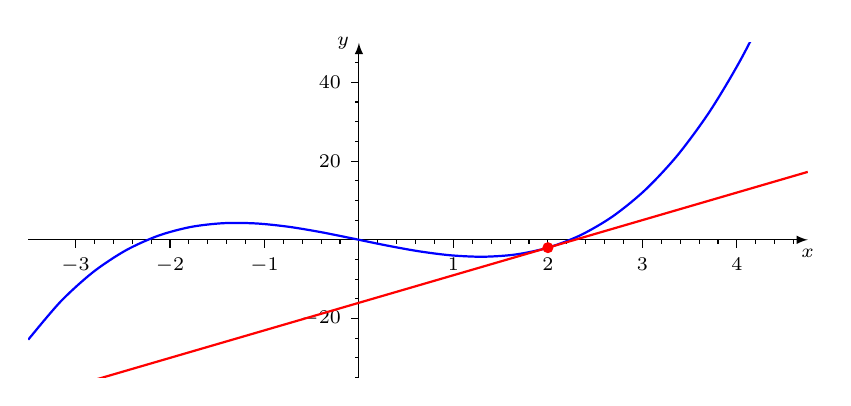
\begin{tikzpicture}[x=12mm,y=0.5mm,>=latex]
          \draw[thin,black,->] (-3.5,0) -- (4.75,0) node[below] {$\scriptstyle{}x$};
          \draw[thin,black,->] (0,-35) -- (0,50) node[left] {$\scriptstyle{}y$};
          % ticks:
          \foreach \x in {-3,-2,-1,1,2,3,4}
          {
            \draw[thin,black] (\x,0) -- (\x,-3pt) node[below] {$\scriptstyle\x$};
          }
          \foreach \x in {-3,-2.8,...,4.6}
          {
            \draw[thin,black] (\x,0) -- (\x,-1.5pt);
          }
          \foreach \y in {-20,20,40}
          {
            \draw[thin,black] (0,\y) -- (-3pt,\y) node[left] {$\scriptstyle\y$};
          }
          \foreach \y in {-35,-30,...,45}
          {
            \draw[thin,black] (0,\y) -- (-1.5pt,\y);
          }
          \begin{scope}
            \clip (-3.5,-35) rectangle (4.75,50);
            \draw[thick,blue,domain=-3.5:4.75,smooth] plot (\x,{(\x)^3-5*\x});
            \uncover<3->{%
              \draw[thick,red,domain=-3.5:4.75,smooth] plot (\x,{7*\x-16});
            }
            \fill[red] (2,-2) circle (2pt);
          \end{scope}
        \end{tikzpicture}
      \end{center}
    }
  \end{enumerate}
  \uncover<4->{\alert{Answer:}\ \answer{D}}

  \vspace*{2in}

}

\end{document}

\frame{
  \frametitle{Review Problems (page 2)}

  \begin{enumerate}
    \setcounter{enumi}{1}
  \item Where is $f(x)=3x^2+12x-4$ decreasing?
    \begin{center}
      A\ $x < -2$
      \quad 
      B\ $x > -2$
      \quad 
      C\ $x < 2$
      \quad 
      D\ $x > 2$
      \quad 
      E\ $x=2$
    \end{center}
  \end{enumerate}
  % \bigskip

  \uncover<2->{%
    \begin{center}
      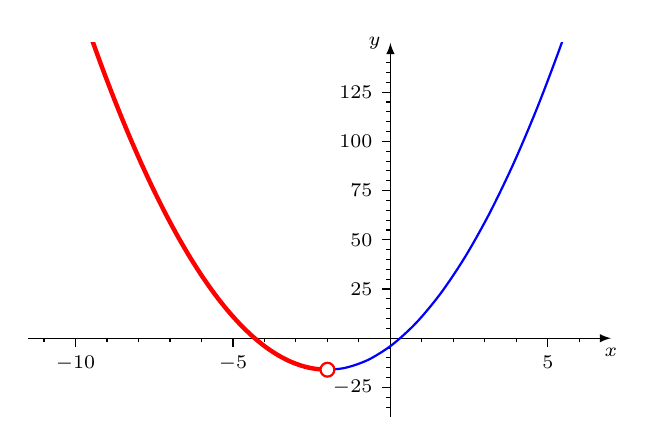
\begin{tikzpicture}[x=4mm,y=0.25mm,>=latex]
        \draw[thin,black,->] (-11.5,0) -- (7,0) node[below] {$\scriptstyle{}x$};
        \draw[thin,black,->] (0,-40) -- (0,150) node[left] {$\scriptstyle{}y$};
        % ticks:
        \foreach \x in {-10,-5,5}
        {
          \draw[thin,black] (\x,0) -- (\x,-3pt) node[below] {$\scriptstyle\x$};
        }
        \foreach \x in {-11,-10,...,6}
        {
          \draw[thin,black] (\x,0) -- (\x,-1.5pt);
        }
        \foreach \y in {-25,25,50,75,100,125}
        {
          \draw[thin,black] (0,\y) -- (-3pt,\y) node[left] {$\scriptstyle\y$};
        }
        \foreach \y in {-35,-30,...,140}
        {
          \draw[thin,black] (0,\y) -- (-1.5pt,\y);
        }
        \begin{scope}
          \clip (-11.5,-40) rectangle (7,150);
          \draw[thick,blue,domain=-11.5:7,smooth] plot (\x,{3*(\x)^2+12*\x-4});
          \uncover<3->{%
            \draw[ultra thick,red,domain=-11.5:-2,smooth] plot (\x,{3*(\x)^2+12*\x-4});
            \draw[thick,red,fill=white] (-2,-16) circle (2.5pt);
          }
        \end{scope}
      \end{tikzpicture}
    \end{center}
  }
  \uncover<4->{\alert{Answer:}\ \answer{A}}

  \vspace*{2in}


}

\frame{
  \frametitle{Review Problems (page 3)}

  \begin{enumerate}
    \setcounter{enumi}{2}
    \item Where is $f(x)=x^3 + 12 x^2 + 6x + 18$ concave up? 
      \begin{center}
        A\ $x< -4$
        \quad 
        B\ $x >-4$
        \quad 
        C\ $x > -2$
        \quad 
        D\ $x < -2$ 
      \end{center}
  \end{enumerate}

  \uncover<2->{%
  \begin{center}
    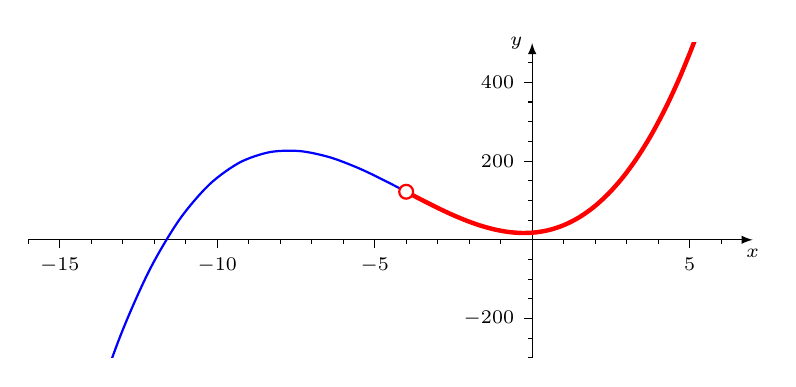
\begin{tikzpicture}[x=4mm,y=0.05mm,>=latex]
      \draw[thin,black,->] (-16,0) -- (7,0) node[below] {$\scriptstyle{}x$};
      \draw[thin,black,->] (0,-300) -- (0,500) node[left] {$\scriptstyle{}y$};
      % ticks:
      \foreach \x in {-15,-10,-5,5}
      {
        \draw[thin,black] (\x,0) -- (\x,-3pt) node[below] {$\scriptstyle\x$};
      }
      \foreach \x in {-16,-15,...,6}
      {
        \draw[thin,black] (\x,0) -- (\x,-1.5pt);
      }
      \foreach \y in {-200,200,400}
      {
        \draw[thin,black] (0,\y) -- (-3pt,\y) node[left] {$\scriptstyle\y$};
      }
      \foreach \y in {-300,-250,...,450}
      {
        \draw[thin,black] (0,\y) -- (-1.5pt,\y);
      }
      \begin{scope}
        \clip (-16,-300) rectangle (7,500);
        \draw[thick,blue,domain=-16:7,smooth] plot (\x,{(\x)^3+12*(\x)^2+6*\x+18});
        \uncover<3->{%
          \draw[ultra thick,red,domain=-4:7,smooth] plot (\x,{(\x)^3+12*(\x)^2+6*\x+18});
          \draw[thick,red,fill=white] (-4,122) circle (2.5pt);
        }
      \end{scope}
    \end{tikzpicture}
  \end{center}
  }
  \uncover<3->{\alert{Answer:}\ \answer{B}}


}
